%%% Thesis Introduction --------------------------------------------------
\chapter{Introduction}
\ifpdf
    \graphicspath{{Introduction/IntroductionFigs/PNG/}{Introduction/IntroductionFigs/PDF/}{Introduction/IntroductionFigs/}}
\else
    \graphicspath{{Introduction/IntroductionFigs/EPS/}{Introduction/IntroductionFigs/}}
\fi

%The Internet has had phenomenal success in the past 20 years, growing from a small research network to a global network that we use in a daily basis. The Internet is logically composed of end hosts interconnected by links and routers. When a host wants to communicate with other hosts, it uses the Internet Protocol (IP) to place information in packets, which are then sent to the nearest router. The router stores, then forwards, packets to the next hop, and through hop-by-hop routing, packets find their way to the desired destination. In other words, end hosts communicate through packet switching. With this communication technique, link bandwidth is shared among all information flows, and so these flows are statistically multiplexed on the link. The resulting service is best effort, in the sense that there are no deterministic guarantees.
%
%Optical burst switching (OBS) is a proposed new communications technology that seeks to expand the use of optical technology in switching systems. Optical technology has been used for a long time to carry information in fibers; however, the rapid growth of the Internet and the progress being made in Dense Wavelength Division Multiplexing (DWDM) creates an opportunity for more extensive use of optical resources in swithching and routing in the second generation of optical network systems. DWDM
%is a fiber-optic transmission technique. It is a multiplexing of many different wavelength signals onto a single fiber to obtain a set of parallel optical channels. Each channel uses a specific wavelength or color. This allows efficient fiber bandwidth and hence, limits the use of additional fibers. 
%
%\begin{figure}[!htbp]
%    \label{fig:trends}
%    \begin{center}
%        \leavevmode
%        \ifpdf
%        \resizebox{120mm}{!}{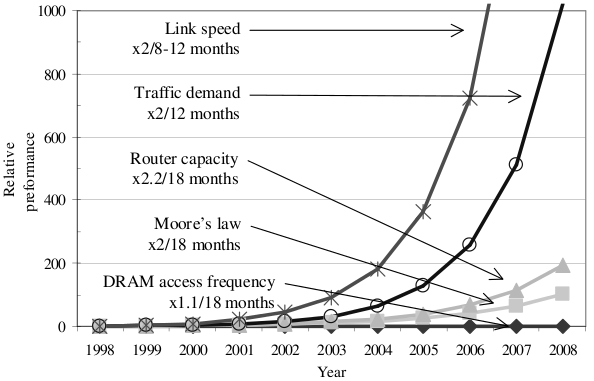
\includegraphics{pmf_thesis_img3}}
%        \else
%        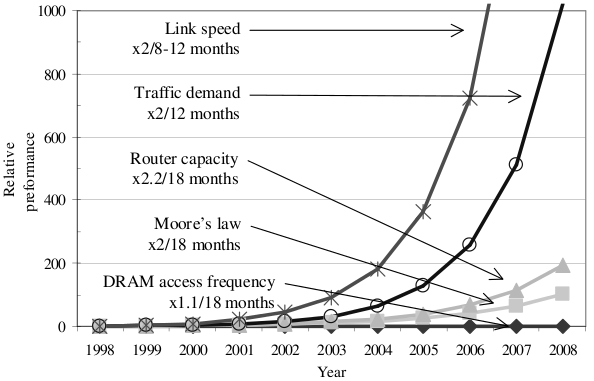
\includegraphics[bb = 92 86 545 742, height=6in]{pmf_thesis_img3}
%        \fi
%        \caption[Trends of traffic demand]{Trends of traffic demand and the underlying technologies in the Internet [1998 = 100\%]. Trends for Silicon processing and router forwarding capacity are kept at the same value as today, despite talks of a slow down after 2004\cite{pablo03}}
%    \end{center}
%\end{figure}
%
%If the Internet is based on packet switching, why would I want to use optical burst switching? The answer is simple. There is a mismatch between the evolution rates of traffic and capacity of the Internet, but optical burst switching can help bridge the gap between demand and supply. recent advances in MEMS \cite{mems}, integrated waveguides \cite{waveguides}, optical gratings \cite{micromirrors}, tunable lasers, and holography have made possible very high capacity switch fabrics. And because of DWDM, single fibers have been able to
%transmit data at speeds up to 400Gb/s. Hence exchange rate will become the bottleneck of network rates \cite{bottleneck}. Optical burst switch network structure proposed in order to exploit the enormous bandwidth of DWDM technology, and overcome the bottleneck of the electron exchange rate.
%
%The novel idea of OBS networks is to keep the information in the optical domain as long as possible. This allows the system to overcome the limitations imposed by the electronic processing and opto-electronic conversion, leading to high speed data forwarding and high transparency. However, many challenging issues have to be solved in order to pave the way for an effective implementation of OBS. Contention, which may occur when two or more bursts compete for the same wavelength on
%the same link, is a critical issue. Many contention resolution methods have been proposed in the literature but many of them are very vulnerable to network load and may suffer severe loss in case of heavy traffic. So we need to develop a new congestion control scheme to prevent congestion collapse and keep OBS network throughput high.
%
\section{About optical burst network}

\begin{figure}[!htbp]
    \label{fig:obstransstep}
    \begin{center}
        \leavevmode
        \ifpdf
        \resizebox{120mm}{!}{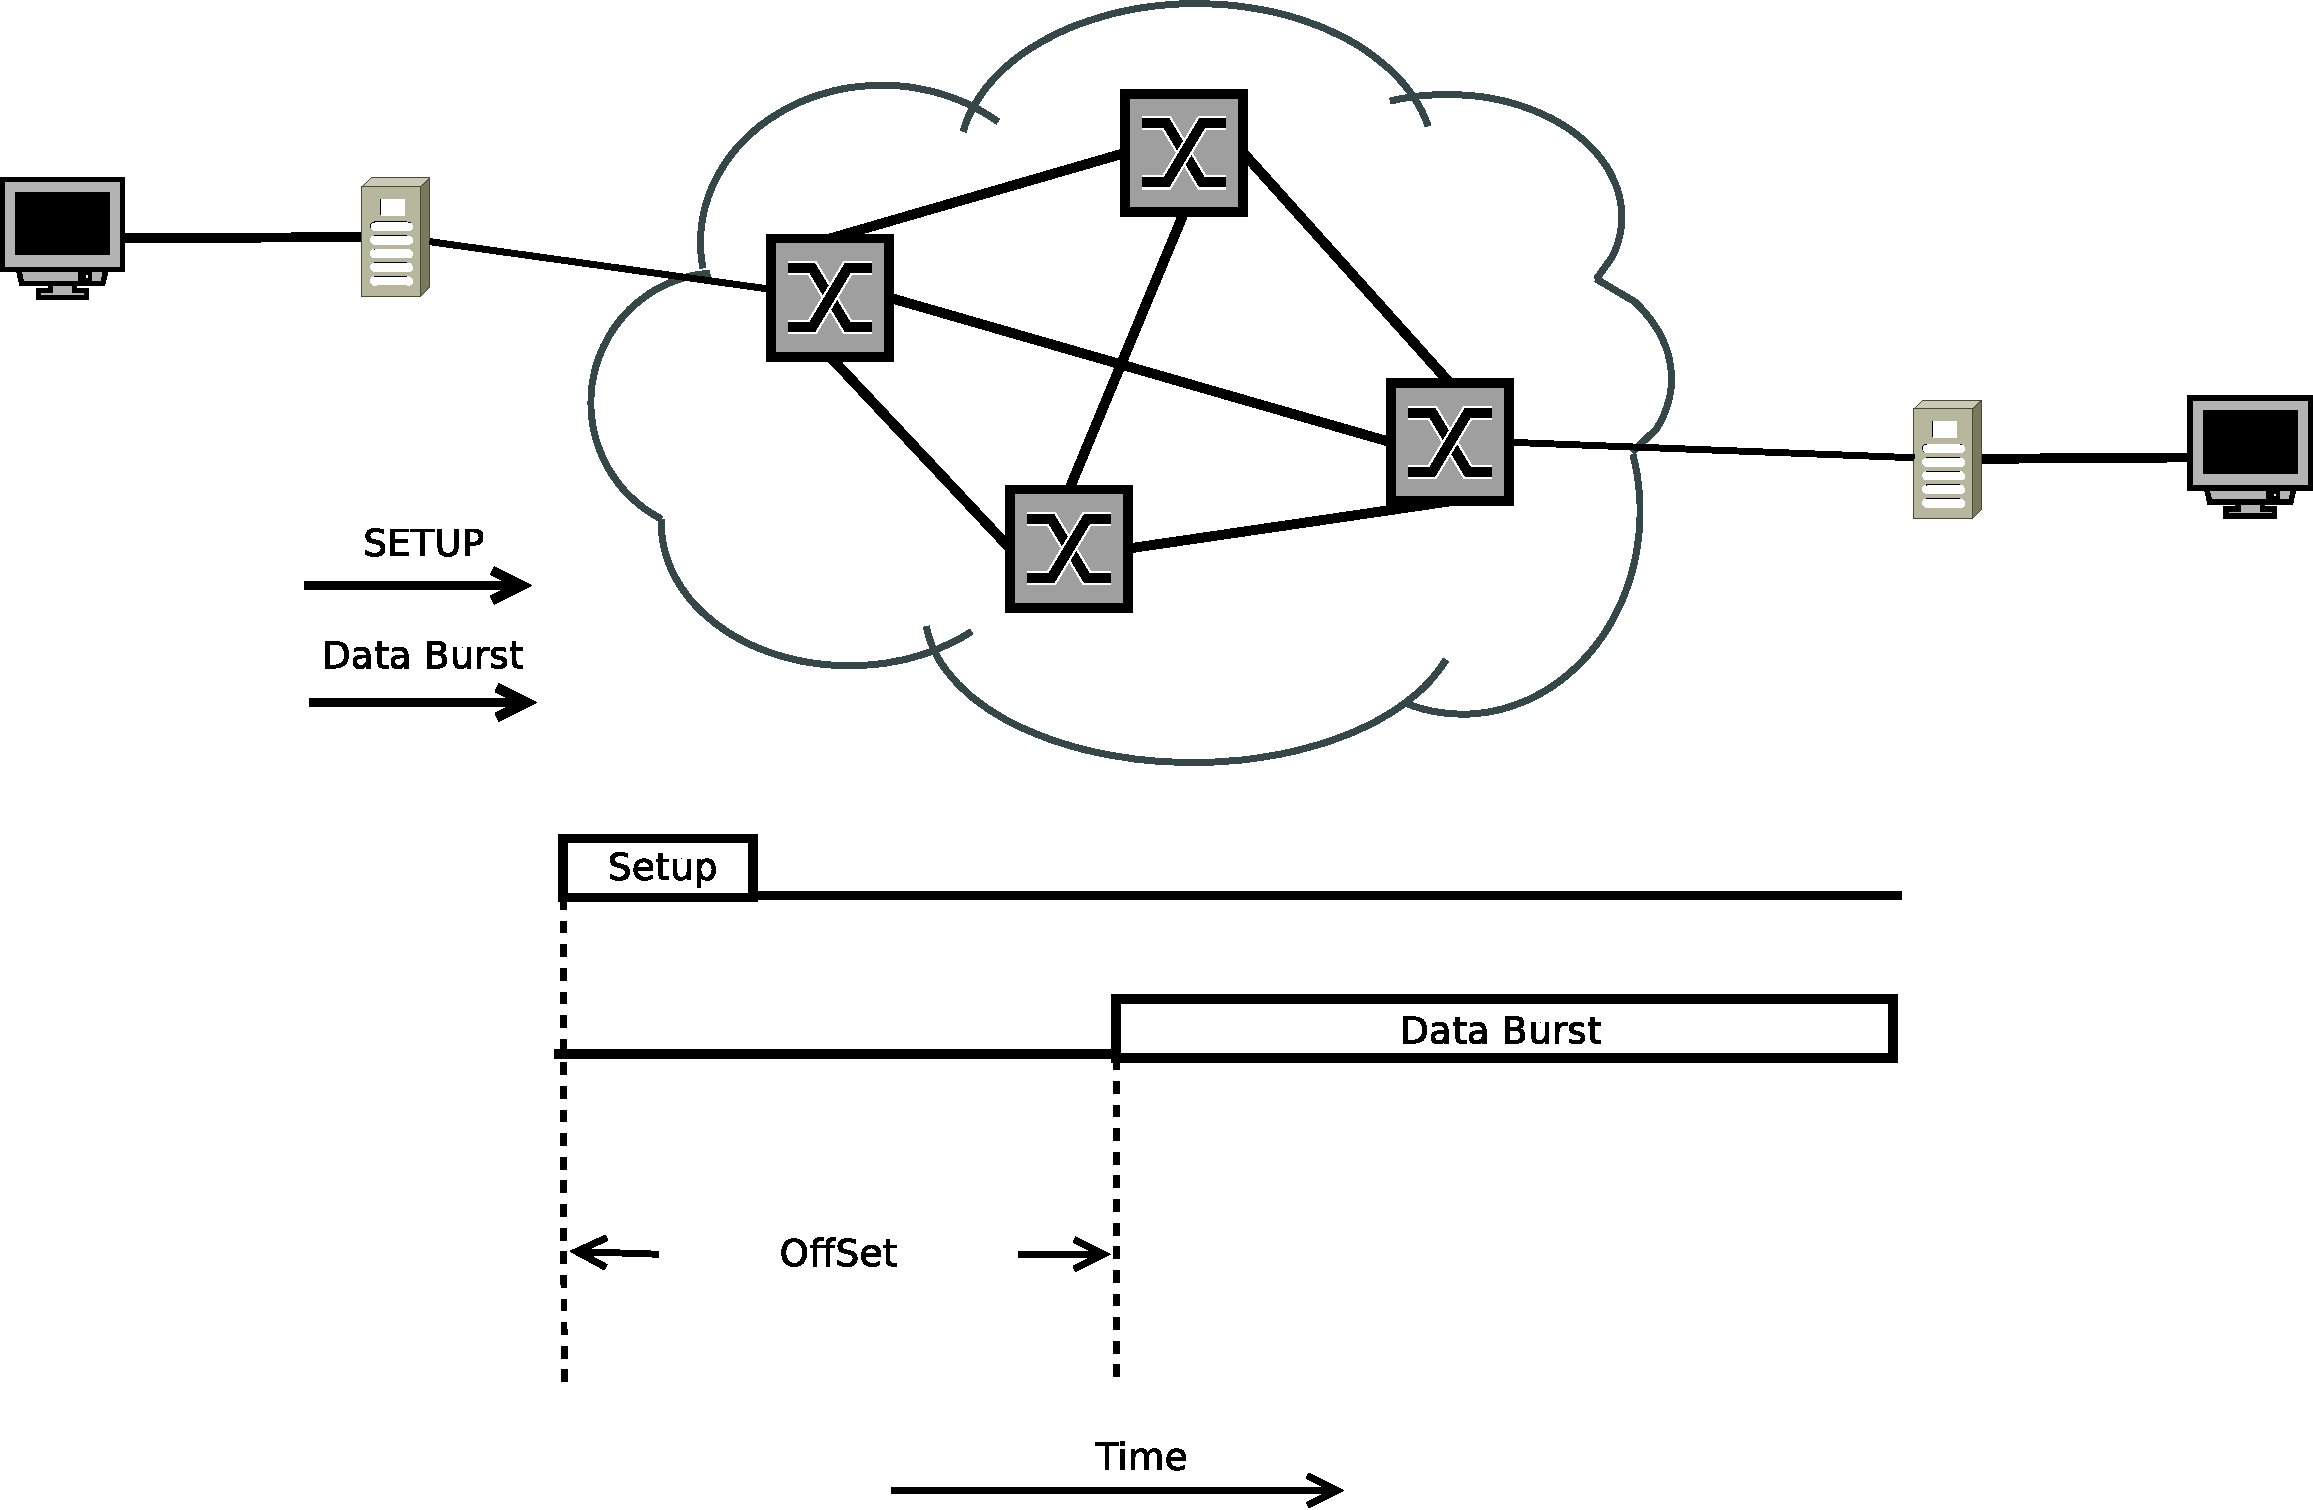
\includegraphics[height=6in]{setup}}
        \else
        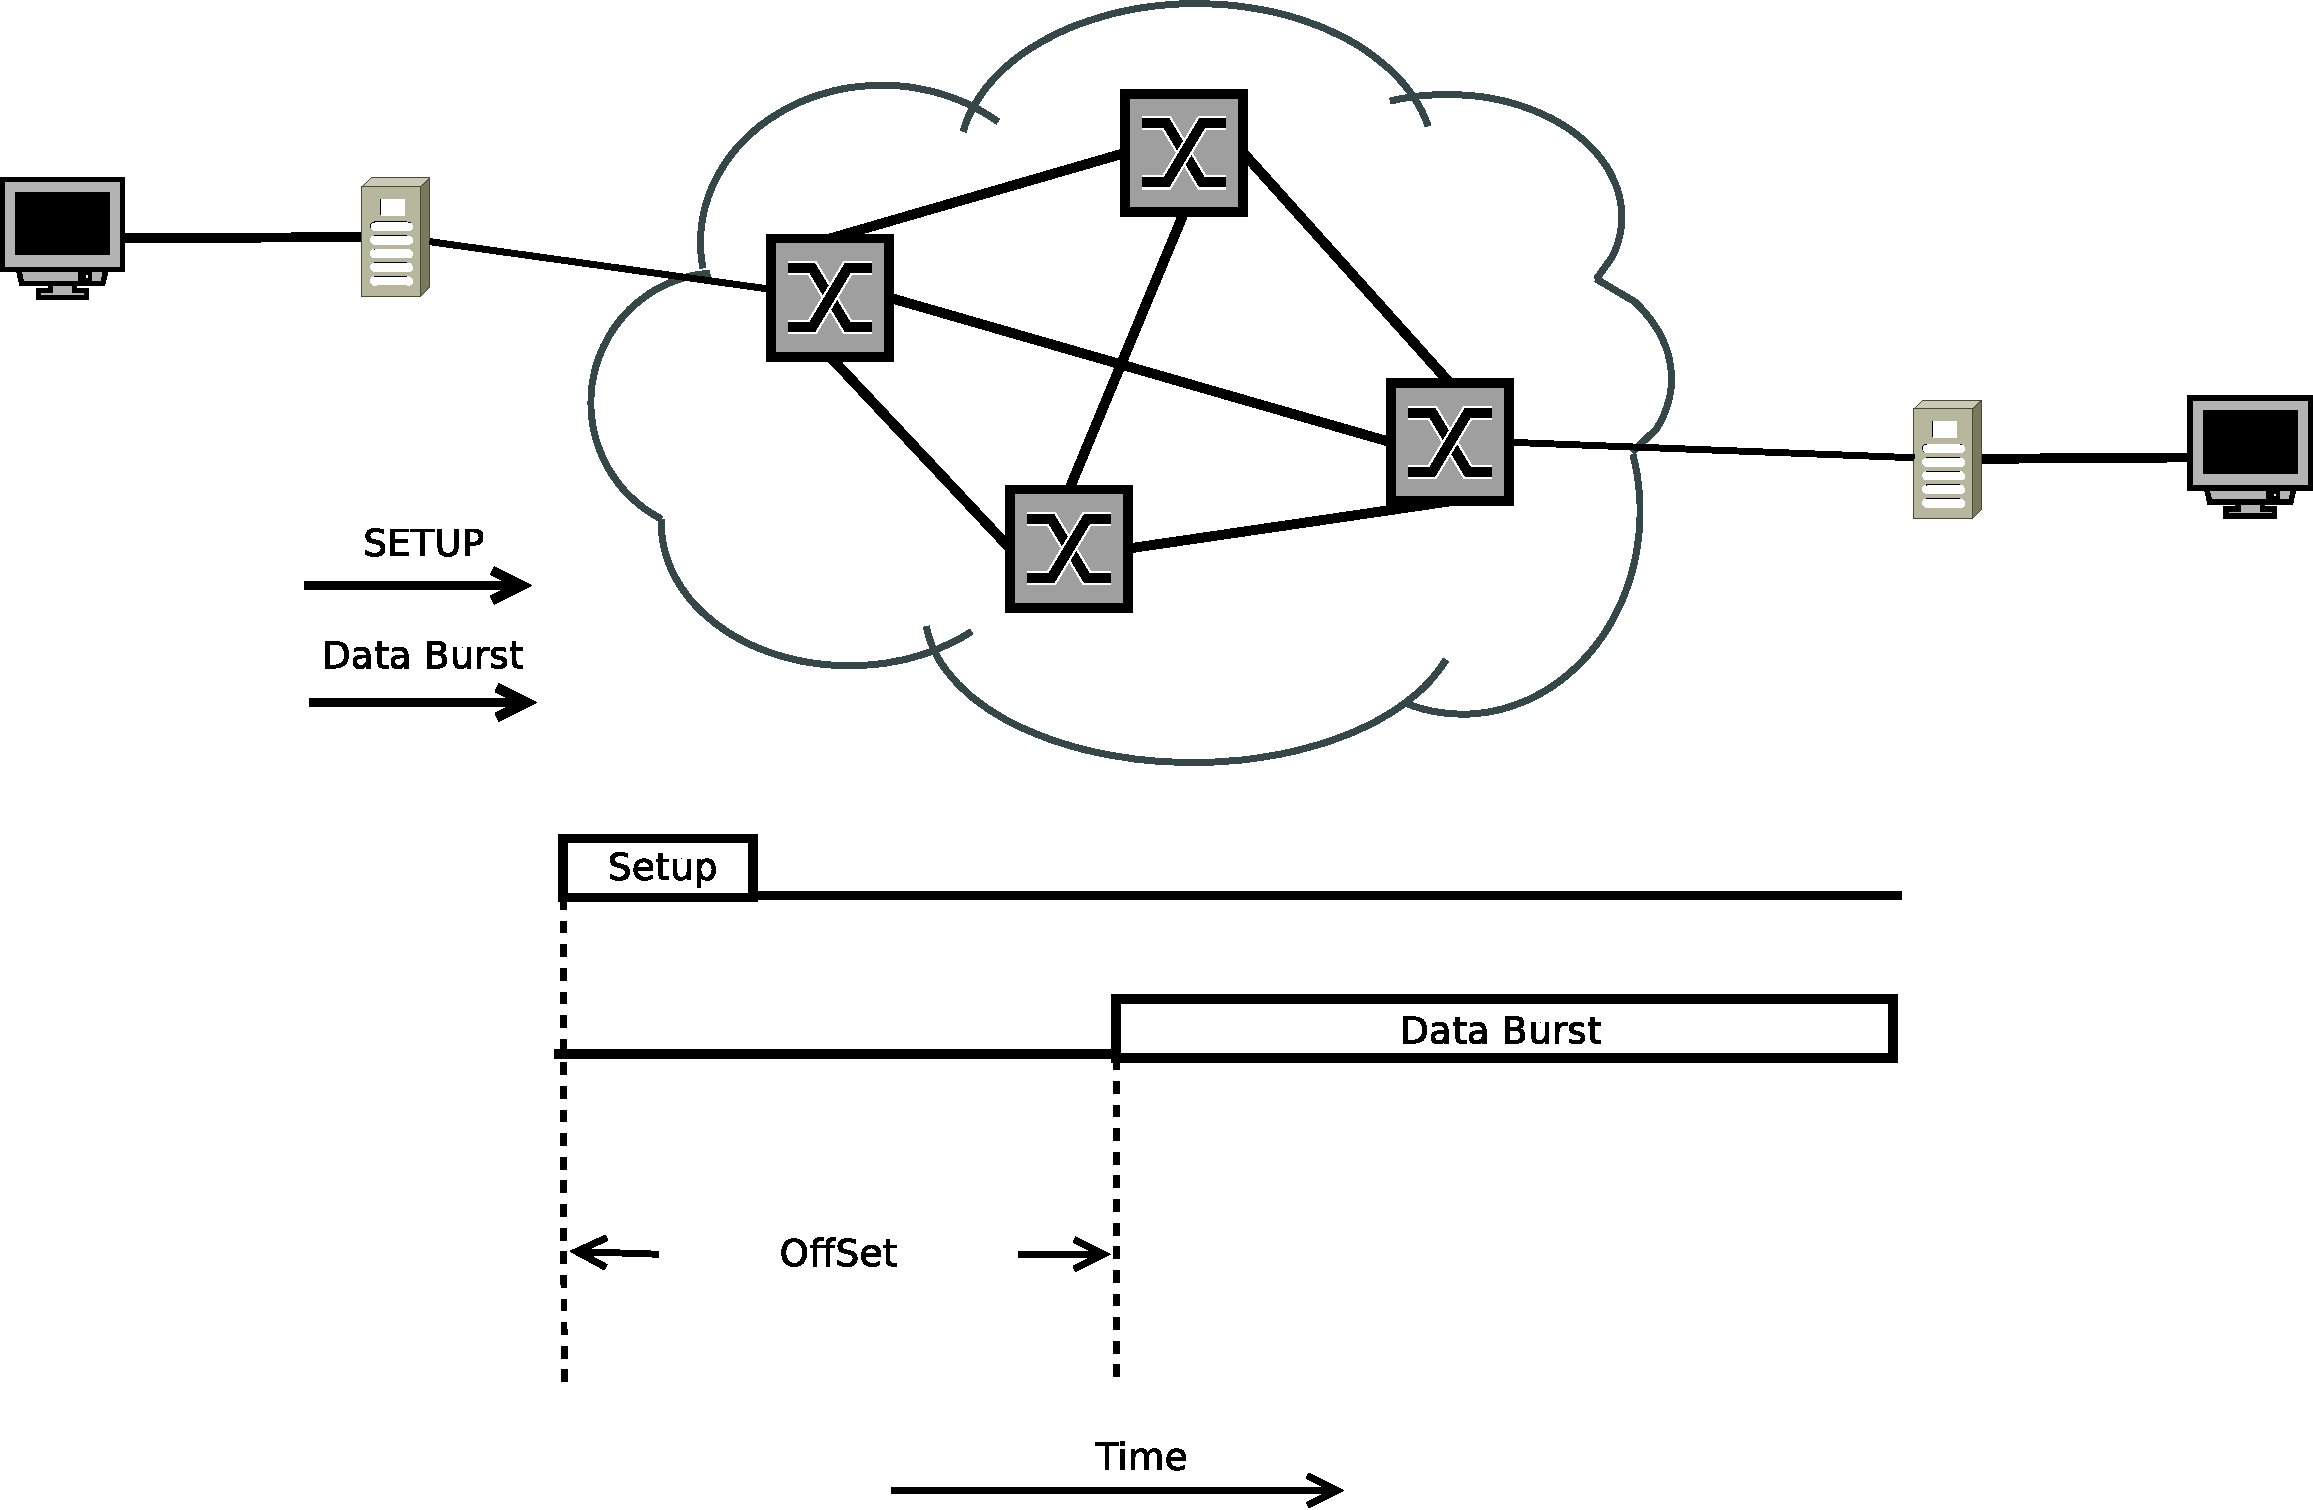
\includegraphics[bb = 92 86 545 742, height=6in]{setup}
        \fi
        \caption{Burst assembly,Burst reservation}
    \end{center}
\end{figure}

Among all optical switching technology, OBS seek to enhance the statistical multiplexing. It has proposed as a new paradigm switching technology for next generation Internet backbone network. Before we get closed to it. We need to get some foundational knowledge, such as what are the big characteristics of this form of exchange of technology. What is the biggest difference compare with traditional switching technology? Does it have born deficiency? 

\begin{figure}[!htb]
    \label{fig:obstime}
    \begin{center}
        \leavevmode
        \ifpdf
        \resizebox{120mm}{!}{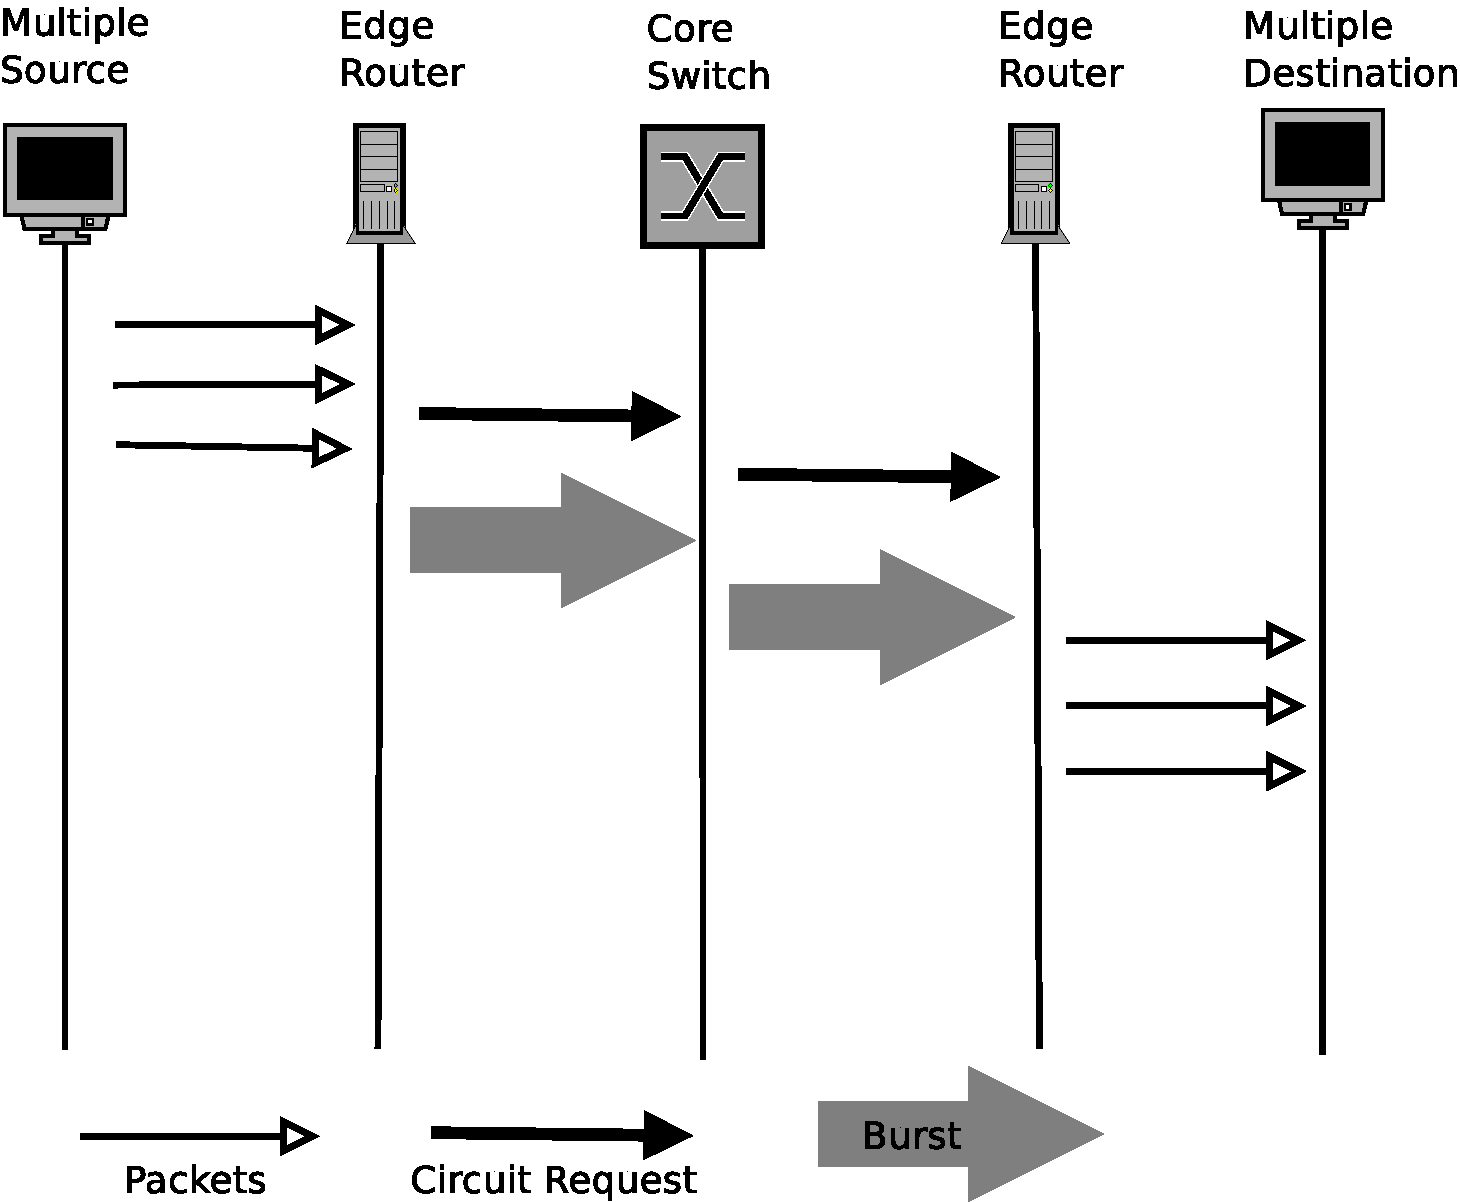
\includegraphics[height=6in]{burst}}
        \else
        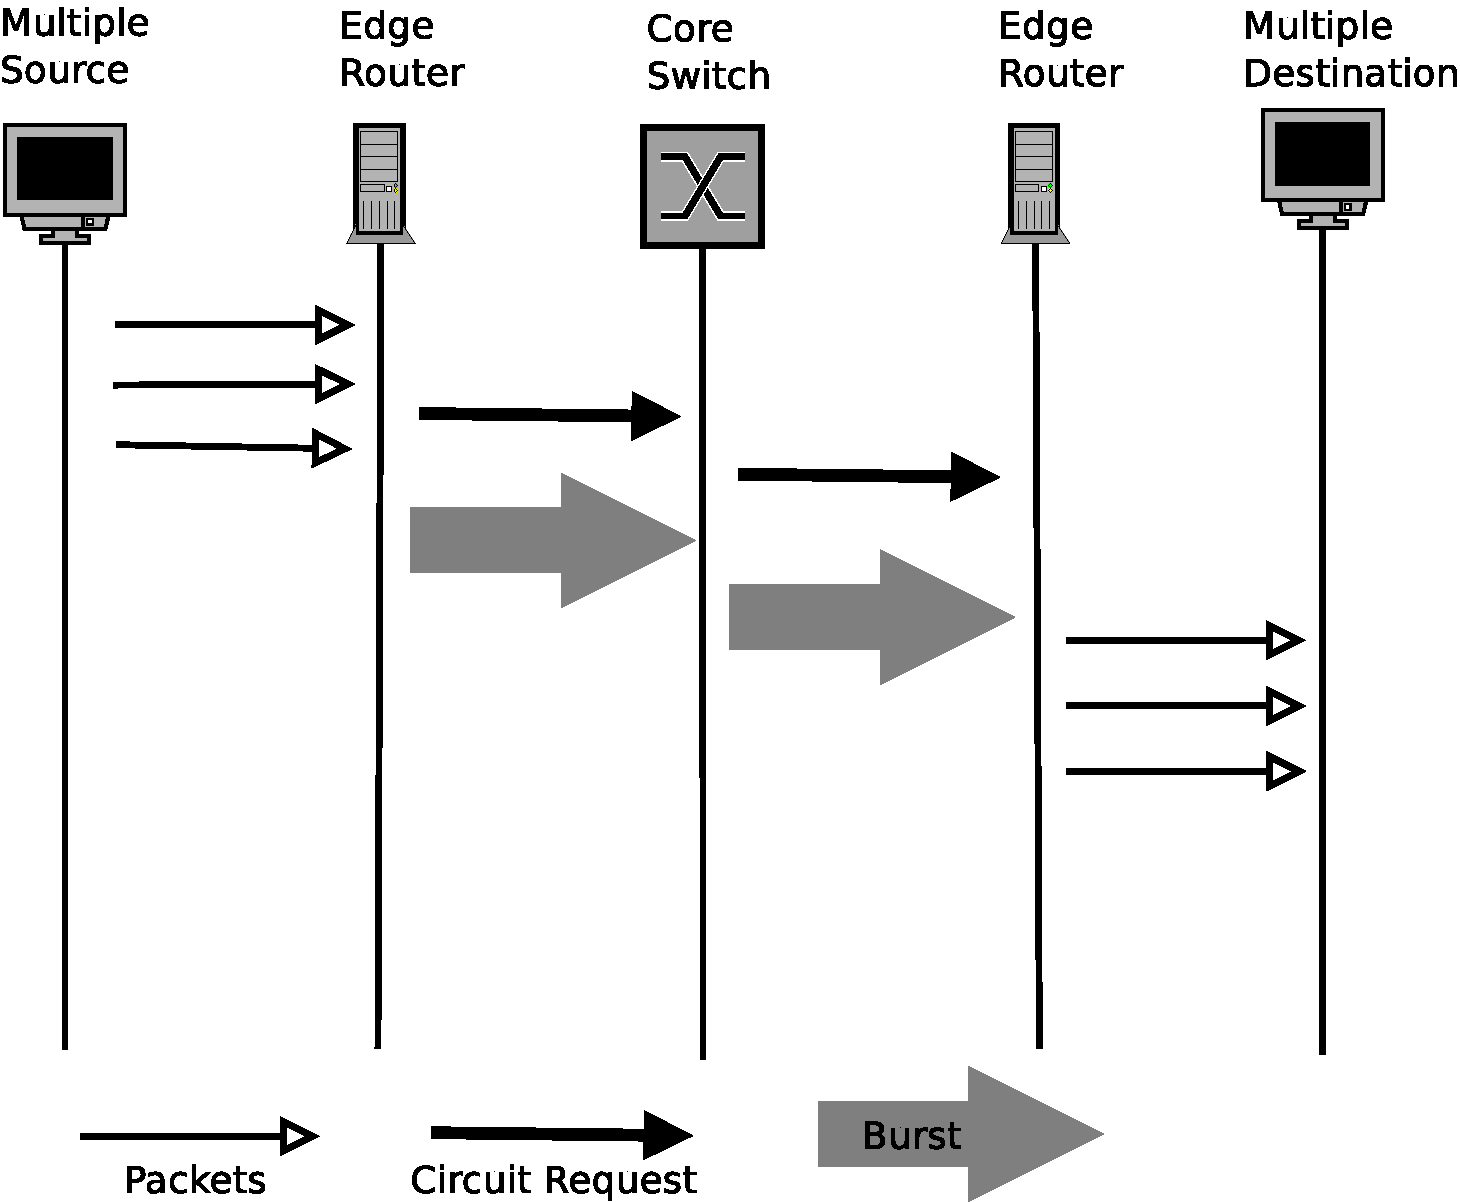
\includegraphics[bb = 92 86 545 742, height=6in]{burst}
        \fi
        \caption{Sample time diagram of a network using OBS}
    \end{center}
\end{figure}

\begin{figure}[!htb]
    \label{fig:burst_format}
    \begin{center}
        \leavevmode
        \ifpdf
        \resizebox{50mm}{!}{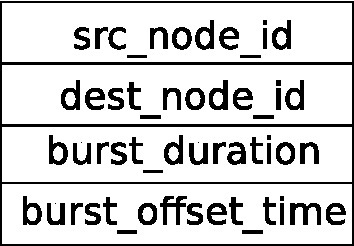
\includegraphics[height=6in]{burst_format}}
        \else
        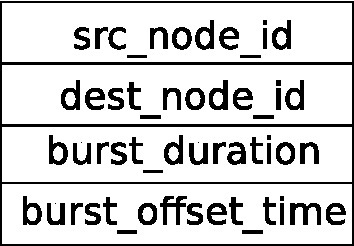
\includegraphics[bb = 92 86 545 742, height=6in]{burst_format}
        \fi
        \caption{OBS burst format sample}
    \end{center}
\end{figure}

The main different compare to conventional packet switching is bufferless on core node. OBS put all intelligent such as buffer, electronic processor, to edge side. As figure \ref{fig:obstransstep} show. All input data bursts are collected into bursts. There may be a classifier to classify packet to different burst according to their destination and Qos requirement or something else. After complete burst assemble and before the burst
transmission begins, a Burst Header Cell (BHC) is sent on the control channel that is separate from data burst channel, carry information about the destination of the burst, duration of the burst, the number of hops it pass through. A sample burst format is shown in figure \ref{fig:burst_format}

A burst switcher, once receiving the BHC, schedule and determine an outgoing link for leading toward the desired destination with an idle channel available, and
then establishes a connection between the channel specified in BHC and the channel through schedule algorithm by core switcher to transmit the burst. It also pass the BHC to next hops on the control channel of the selected link. After the core router prepare for arriving burst, the burst go through core router without additional operation. It also refer as one-way reservation. The burst just wait a certain offset time and don't need to check the ACK from reservation process. Once
burst arrive to core router, It can be transmit in whole optical domain. That is the reason why OBS better than others mechanism. The mechanism for resource reservation and release has been study for a long time. In simple term, There are four major combinations as table \ref{tab:setupclass} show.

\begin{table}[!htbp]
    \label{tab:setupclass}
    \centering
    \setlength{\extrarowheight}{1mm}
    \addtolength{\tabcolsep}{3mm}
    \begin{tabular}{|r|l|l|}
        \hline
        \backslashbox{release}{setup} & Immediate setup & Delay setup \\
        \hline
        \multirow{2}{*}{Immediate release} & Immediate setup & Delay setup\\
                                           & Immediate release & Immediate release\\
        \hline  
        \multirow{2}{*}{Explicit release} & Immediate setup& Delay setup \\
                                          & Explicit release & Explicit release \\
        \hline
    \end{tabular}
    \caption{Classification of reservation/release schemes}
\end{table}

There are two main scheduling mechanism, that is so called \verb|LAUC| and \verb|LAUC-VF|, \verb|LAUC| is abbreviation of First-Fit, Horizon, Latest Available Unscheduled Channel. And \verb|LAUC-VF| is abbreviation of \verb|LAUC| with Void Filling. Since \verb|LAUC-VF| is the improvement of \verb|LAUC|, I employ \verb|LAUC-VF| algorithm in simulation.


\section{Finding \& Trends}
As we know, in \verb|OBS|, all intelligence resides in the edge nodes, which are at the same time the buffer and the processor on the network.     Simply put, current congestion control scheme are same pattern. They all gathering network state information first. Setup a certain threshold to estimate the congestion state. And then send a customize message to edge router according to the current network state. 


\begin{figure}[!htb]
    \label{fig:pattern}
    \begin{center}
        \leavevmode
        \ifpdf
        \resizebox{120mm}{!}{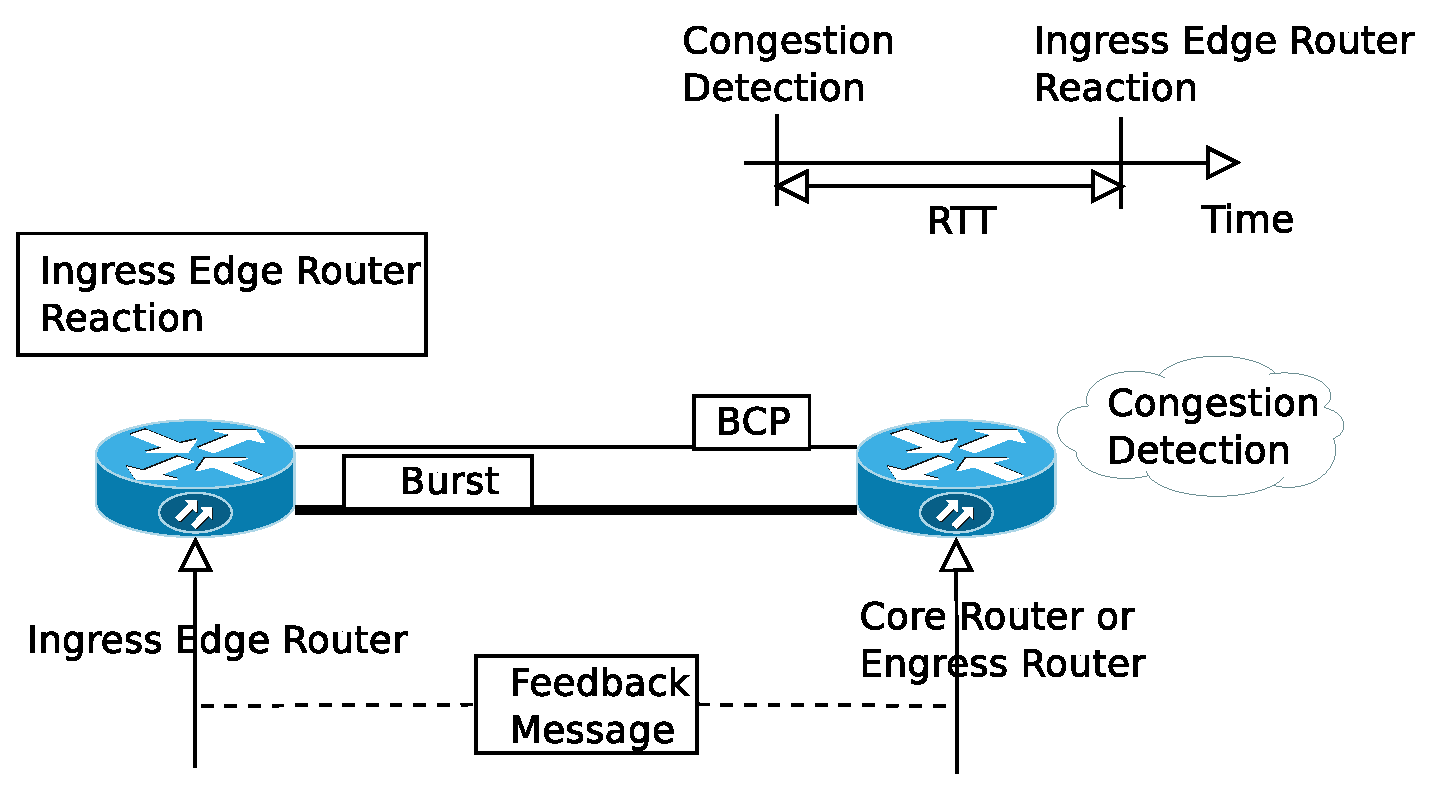
\includegraphics[height=6in]{pattern}}
        \else
        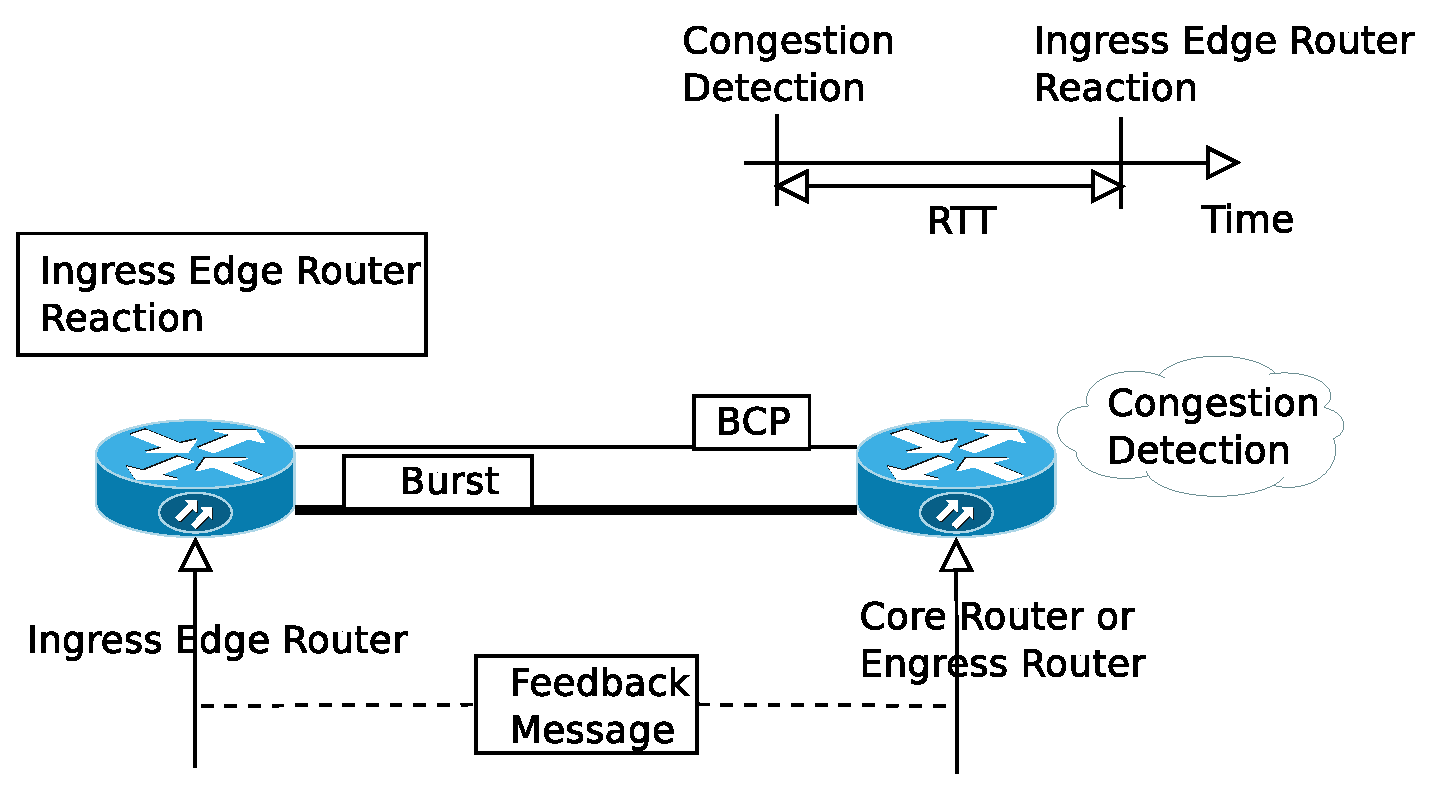
\includegraphics[bb = 92 86 545 742, height=6in]{pattern}
        \fi
        \caption{Pattern to control OBS congestion}
    \end{center}
\end{figure}

Figure \ref{fig:pattern} not only tell us the current popular pattern on research about OBS congestion control. It also tell us the steps to control congestion. This patter is practical and correct. So it will also be used in this study. Although the petter of vary congestion control mechanism are same. But there are a large amount difference among vary scheme in implementation detail. Such as different frequently to send feedback message to edge router, different way to
determine the congestion state threshold, different feedback message body. Certainly, they result in different performance. 

In their paper, they don't tell how to setup the threshold. They just give a final result. The value maybe have test a lot of times and they think that is proper for their model. It also is a constant value. But I think this value should adjust with the change of network topology. Besides, They don't tell how long is the RTT. The \verb|RTT| can use to measure the speed of ingress react. The \verb|Threshold| is a most important factor to affect the scheme to indicate congestion state or not.
But there is not a formula to got these two value through pure analysis. Current scheme just by trial and error to find a proper value for their simulation model.  

Moreover, Once their model is determined. All parameter is definite during simulation time. Include the most important \verb|Threshold| value. In my opinion, Congestion control is a dynamic optimization problem. This \verb|Threshold| should self-adjust accordingly. Burak Kantarci and Sema Oktug propose a congestion control scheme base on adaptive threshold \cite{adaptive}. The improvement is also very good. 

The previous researcher use throughput and loss ratio to measure their result. The higher throughput and the lower loss ratio. That will be propose as a better congestion control scheme. There also very important factor should be consider to determine whether a new scheme is better. That is whether as effective at high load as at low load. All previous researcher have pay much attention to this point. 

Previous mostly assume the burst arrive process follow the Poisson process and their lengths are negative exponentially distributed. But base on the some newest study. It has been shown that  whereas flow arrivals are Possion (or close to Possion), flow sizes are not exponential, but rather heavy-tailed, and thus they are closer to a Pareto distribution than an exponential one.  

\section{Issues May Encounter}

Note that in OBS networks, intelligent functions such as burst assembly, burst scheduling and generation of control packets are implemented at edge nodes while core nodes perform less complex functions such as processing control packets, resource reservation and switching bursts. However, many existing works have proposed to implementation some simple extra functions at the core node such as load calculation, burst segmentation and priority-based burst dropping for service differentiation.
It is hard to predict whether it is necessary to add extra function to core node in this study. If yes, is it complicate so that the core node is reject to add it.


To meet QoS requirement such as bounded delay or guaranteed delivery is part of new scheme objective. But it is incompatible to achieve guaranteed delivery rate and congestion control by reduce transmission rate at the same time. It is clear that even in ideal networks, where the switches use number of buffers and can perform wavelength conversion, congestion collapse still occurs when the load gets higher. On this moment, it seem impossible to resolve this contradiction.    

\section{Summary}

Overview the history of the development of OBS technology. The original goal is to compete with ATM network which have great potential in electronic domain. Compared with primitive Burst switching, ATM is more cost effective. But when WDM technology can provide huge bandwidth. It posed a challenge to current switch technology, that is how to use this bandwidth efficiently. The switch technology become the network bottleneck. OBS is a new technology that is currently
under study. It has not as yet been commercialized and standardized. But It has great potential to replace current switch technology. It has some advantages:

\begin{enumerate}
    \item More flexible and efficient compared with wavelength routed network
    \item More scalable and cost effective compared with opto-electronic approaches
    \item Smaller overhead and more practical compared with OPS
\end{enumerate}

It also have some prominent feature:

\begin{enumerate}

    \item Separation of transmission and control, Each user transmits data in bursts
    \item Basically, assumes the network is bufferless
    \item Network nodes(OXC) allocate resources for just this single burst

\end{enumerate}

By contrast, we can find that OBS has a lot of advantages for packet switch. However, unfortunately contention is inherent to the OBS technique. The contention problem is due to the lack of information at the nodes and the absence of global coordination between the edge routers and core routers. In one word, I want to proposed a new scheme to avoid and control congestion effectively in this study. And then drive OBS into standardized earlier.



%%% ----------------------------------------------------------------------


%%% Local Variables: 
%%% mode: latex
%%% TeX-master: "../thesis"
%%% End: 
